\documentclass{ctexart}
\CTEXsetup[format={\Large\bfseries}]{section}            % 让section靠左对齐
\usepackage{graphicx} % Required for inserting images
\usepackage{enumerate} % 下面1,2,3小点
\usepackage{subcaption}

% 设置 subsection 的间距
\usepackage{titlesec}
\titlespacing{\section}{0pt}{0.75\baselineskip}{0.75\baselineskip}
\titlespacing{\subsection}{0pt}{0.5\baselineskip}{0.5\baselineskip}

\usepackage{geometry} % 调整页边距和纸张大小
\geometry{a4paper,scale=0.7} 

\title{\vspace{-2cm}\textbf{程序设计基础课程设计报告} \\ \fontsize{12}{14}{---模拟图书馆管理系统}}

\author{高宇轩 23009200132}
\date{\today}

\begin{document}
    
    \maketitle
    
    \section{原始题目及要求}
    编写一个程序模拟图书管理系统。用户分为管理员和读者两类,分别显示不同文本格式菜单,通过菜单项对应数字进行选择。读者菜单包括借书、还书、查询等功能。管理员菜单包括图书和读者信息录入、修改和删除。图书信息至少应包括:编号、书名、数量,读者信息至少应包括:编号、姓名、所借图书。可根据图书名称或编号进行图书信息查询,可查询某本书现在被哪些读者借走。
    
    命令行参数如下:
    Libsim –a(-u) xxxx
    
    第一个参数为可执行程序名称;
    
    第二个参数为用户身份,-a表示管理员,-u表示读者;
    
    第三个参数为用户名。

    
    \section{题目分析}
    
    \subsection{题目功能}
    读者:可以借书,还书,查询图书馆有的书籍,查阅已经借阅的书籍。
    
    管理员:能够录入、修改和删除图书信息、读者信息。
    
    \subsection{题目知识点}
    文件读写、内存管理、结构体定义、基本数据结构、高级格式化输入输出。
    
    \section{题目总体方案设计}
    
    \subsection{程序包含的模块结构图}
    程序主要包括BookShelf和UserLists两个数据库,管理员的录入、修改与删除,用户的借书、还书、查询信息都是基于这两个数据库进行操作的。
    
    \begin{figure}[h] % 'h' 表示将图片放置在当前位置
        \centering
        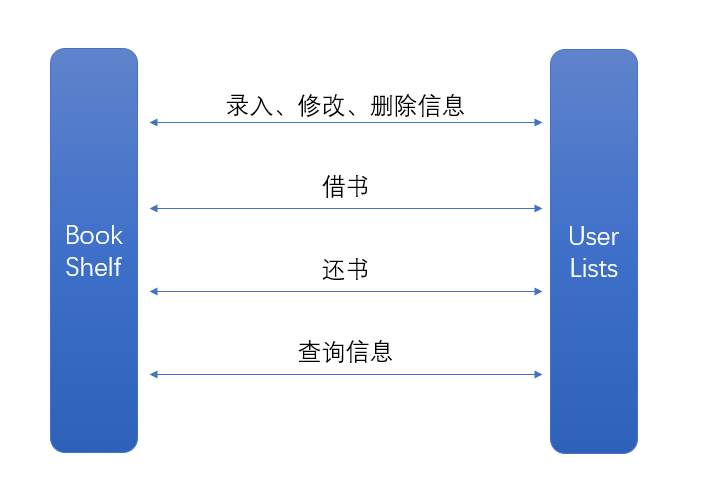
\includegraphics[width=0.75\textwidth]{src/modules.png}
        \caption{程序的模块结构图}   
    \end{figure}
    
    \subsection{输入输出数据说明}
    在命令行中输入 Libsim –a(-u) xxxx,根据用户身份,输出不同的功能菜单,包括功能和对应的数字选项。
    
    如果是读者,在借书、还书或者查询书籍时,要求用户输入对应的书籍名称,输出借书、还书或者查询书籍是否成功,并输出对应书籍的信息;在查询用户自身的借阅信息时,输出用户已经借阅的书籍信息。
    
    如果是管理员,如果录入书籍或读者信息,提示管理员用指定的格式输入信息,输出是否录入是否成功,同时输出新录入的数据信息;如果修改书籍或读者信息,让管理员选择信息的种类并输入,输出修改是否成功,同时输出修改后的数据信息;如果删除书籍或读者信息,提示管理员输入对应的名称,输出删除是否成功。
    
    
    \subsection{数据结构说明}
    使用bookshelf和userlist两个链表分别存储和维护书籍信息与用户信息。
    
    使用Book结构体存储书籍信息,包括string类型的图书编号,string类型的图书名称,int类型的图书数量,int类型的可借阅数量,pair<string, string>*类型的借阅用户编号与用户名称。
    
    使用User结构体存储用户信息,包括string类型的用户编号,string类型的用户名称,int类型的借书数量,pair<string, string>*类型的借阅书籍编号与书籍名称。
    
    \begin{figure}[h] % 'h' 表示将图片放置在当前位置
        \centering
        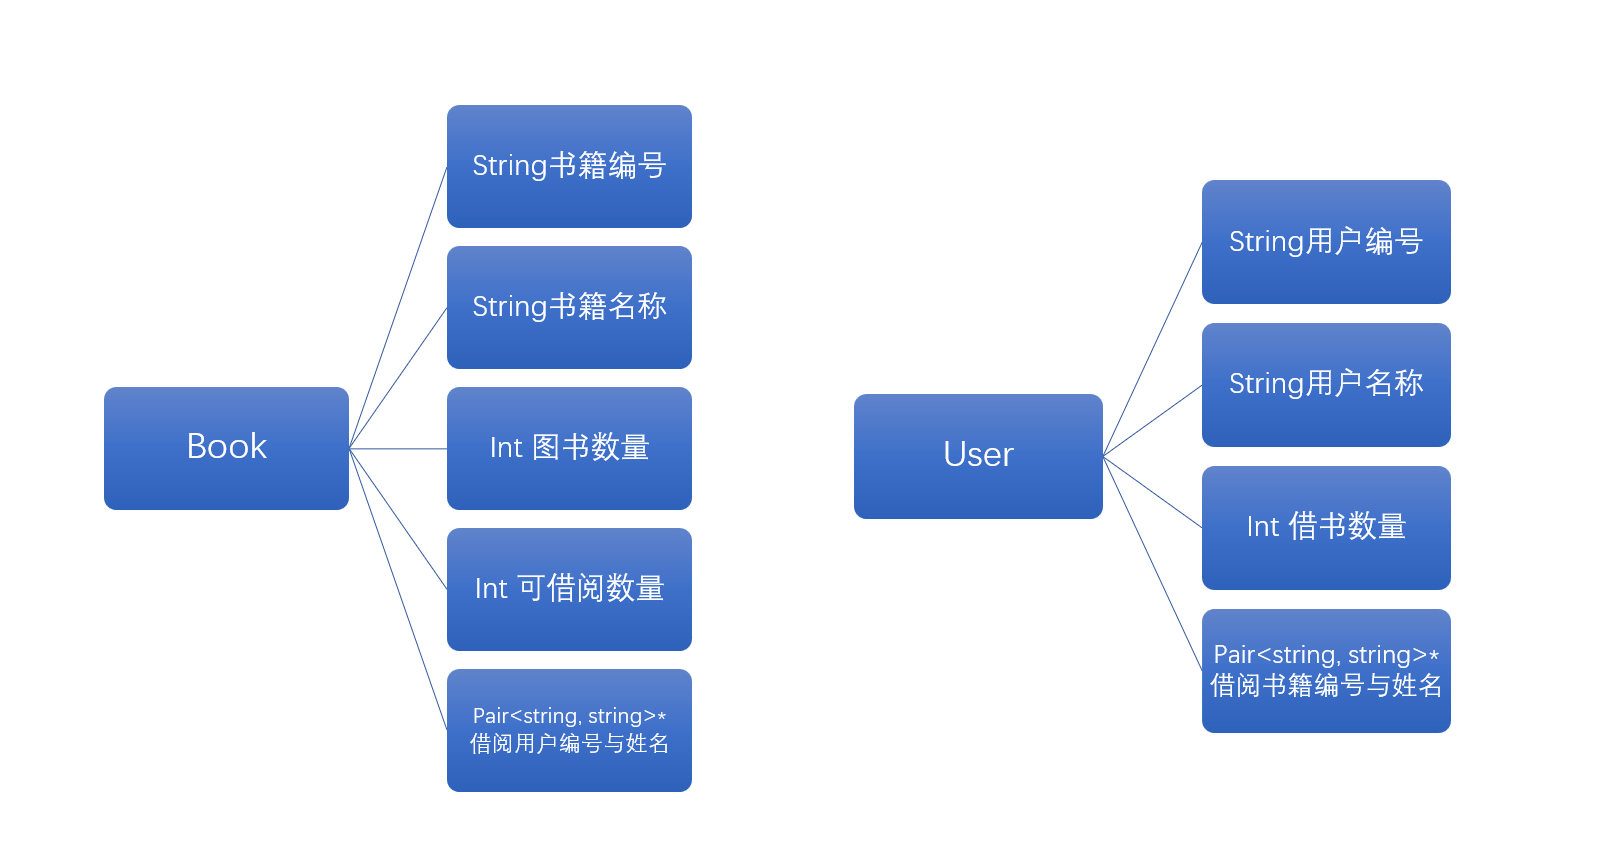
\includegraphics[width=1\textwidth]{src/structs.png}
        \caption{Book和User的struct示意图}    
    \end{figure}
    
    \subsection{程序功能流程图}
    以下是用户与管理员操作的主要流程图
    
    \begin{figure}[h]
        \begin{minipage}[t]{0.5\linewidth}
            \centering
            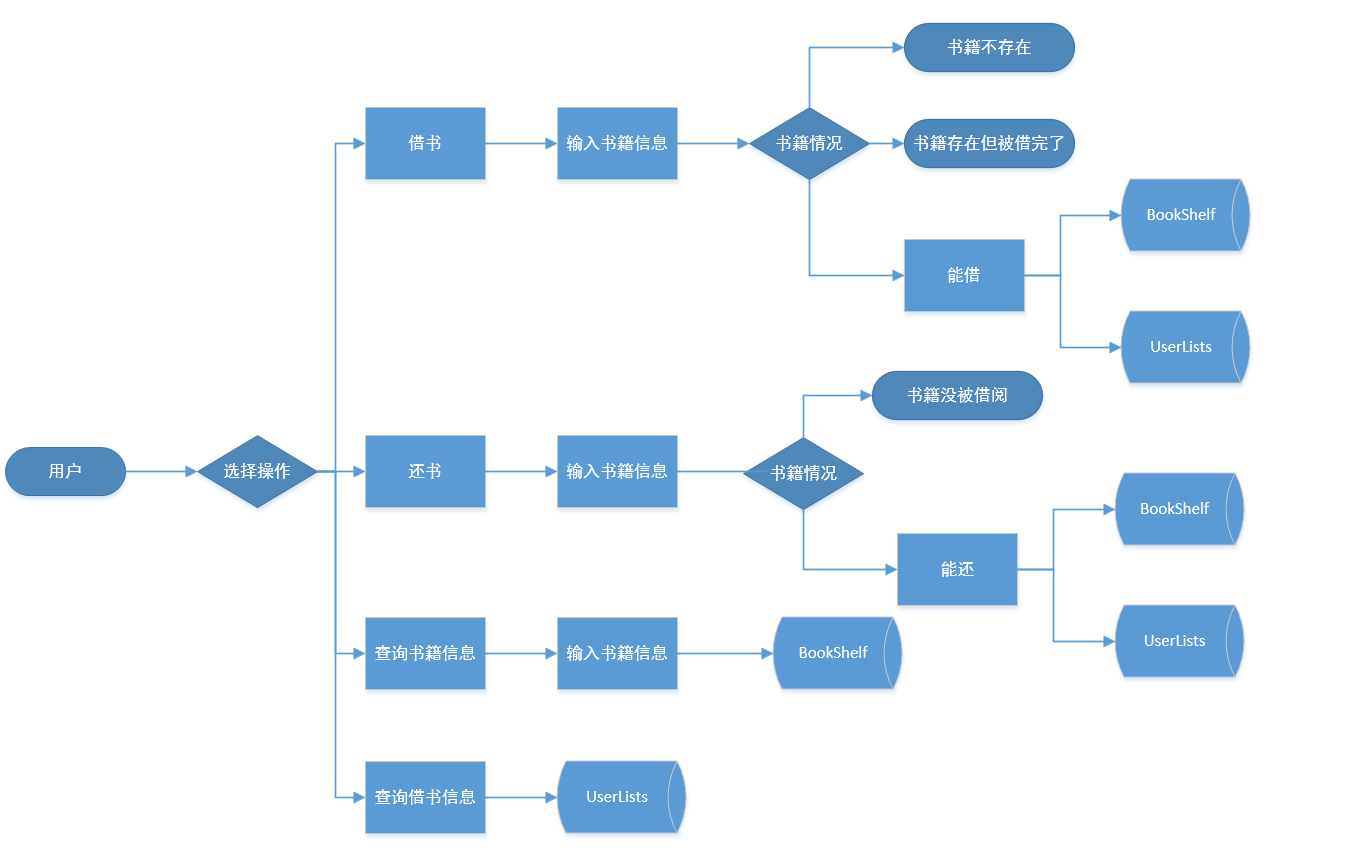
\includegraphics[width=\linewidth]{src/user.png}
            \caption{用户操作流程图}
        \end{minipage}%
        \begin{minipage}[t]{0.5\linewidth}
            \centering
            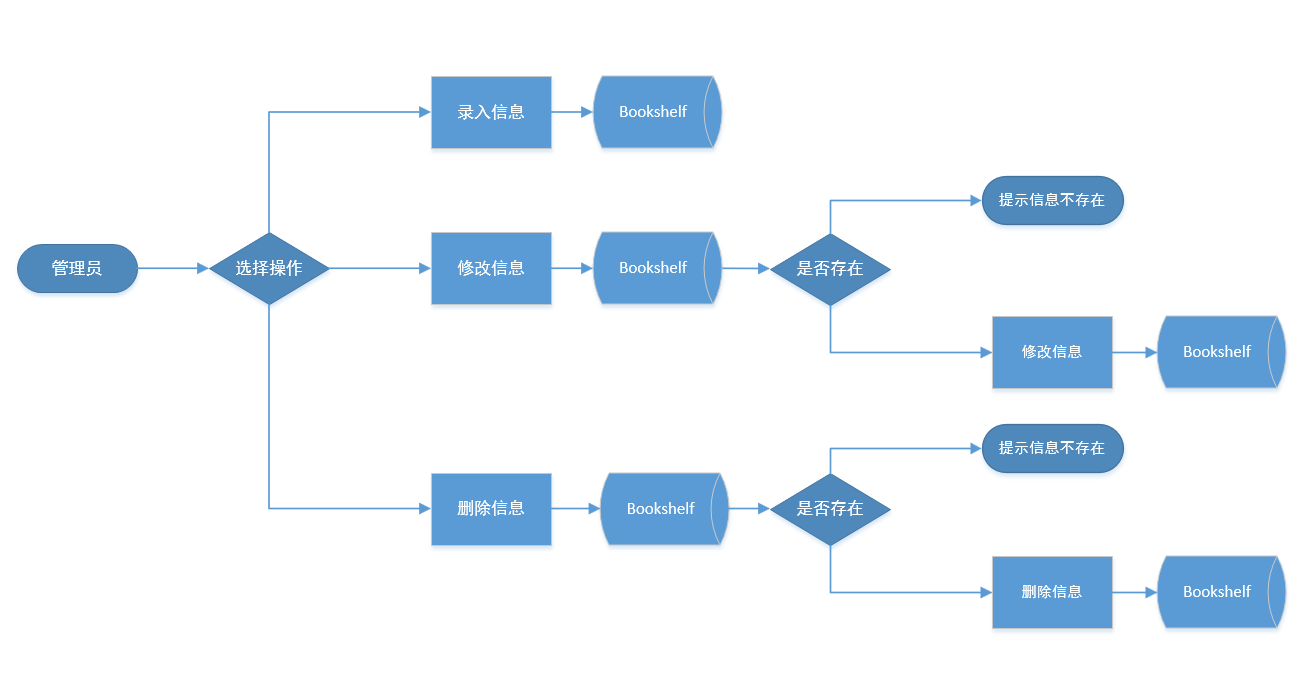
\includegraphics[width=\linewidth]{src/admin.png}
            \caption{管理员操作流程图}
        \end{minipage}
    \end{figure}
    
    
    \section{各功能模块的设计说明}
    \subsection{数据库}
    因为数据不可能一直存储在程序中,所以要把数据存在外部的文件中,每次打开程序时从外部文件载入数据,结束程序时将数据重新写入外部数据文件。
    
    因此,我们创建对应的books\_info.txt, users\_info.txt, borrow\_info.txt三个文件,分别存储书籍信息,用户信息以及借阅情况。
    
    books\_info.txt中存储的是书籍信息,每一行代表一种书。一行中有4个用空格分隔的字符串,分别代表书籍编号、书籍名称、图书数量与可借阅数量,其中书籍名称中如果包含空格,用下划线\_代替,防止程序出错。
    
    users\_info.txt中存储的是用户信息,每一行代表一个用户。一行中有3个用空格分隔的字符串,分别代表用户编号,用户名称和已借阅数量,其中用户名称中如果包含空格,用下划线\_代替,防止程序出错。
    
    borrow\_info.txt中存储的是借阅信息,每一行代表一次借阅操作。一行中有4个用空格分隔的字符串,分别代表被借阅的书籍编号、被借阅的书籍名称、借阅者的用户编号,借阅者的用户名称。其中书籍名称或者用户名称中如果包含空格,同样用下划线\_代替,防止程序出错。
    
    
    \subsection{借书、还书与查询信息}
    借书时,根据用户输入的书籍信息,先判断书籍与用户是否存在以及能否被借阅,然后分别修改书籍的可借阅数量,借阅用户编号与姓名,用户的借书数量,借阅书籍编号与姓名。
    
    还书时,根据用户输入的书籍信息,先判断用户是否借阅了该书籍,然后分别修改书籍的可借阅数量,借阅用户编号与姓名,用户的借书数量,借阅书籍编号与姓名。
    
    查询书籍信息与用户借书信息时,先判断书籍或者用户信息是否存在,然后输出书籍或者用户的借阅或被借阅情况。
    
    
    \section{程序的集成测试}
    在程序的集成测试中,我们依次对管理员的每一个选项进行操作,然后对用户的每一个选项进行操作,以下是程序的测试信息。
    
    图5是运行程序前,数据库中的信息;
    
    图6是以管理员身份开始运行程序时的界面;
    
    图7是用管理员身份进行的操作;
    
    图8是以管理员身份操作之后的数据库信息;
    
    图9是管理员运行程序后,数据库中的信息;
    
    图10是以用户身份开始运行程序时的界面;
    
    图11是以用户身份进行的操作;
    
    图12是用户运行程序后,数据库中的信息;
    
    \vspace{2em}
        
    \begin{figure}[!htbp] % 'h' 表示将图片放置在当前位置
        \centering
        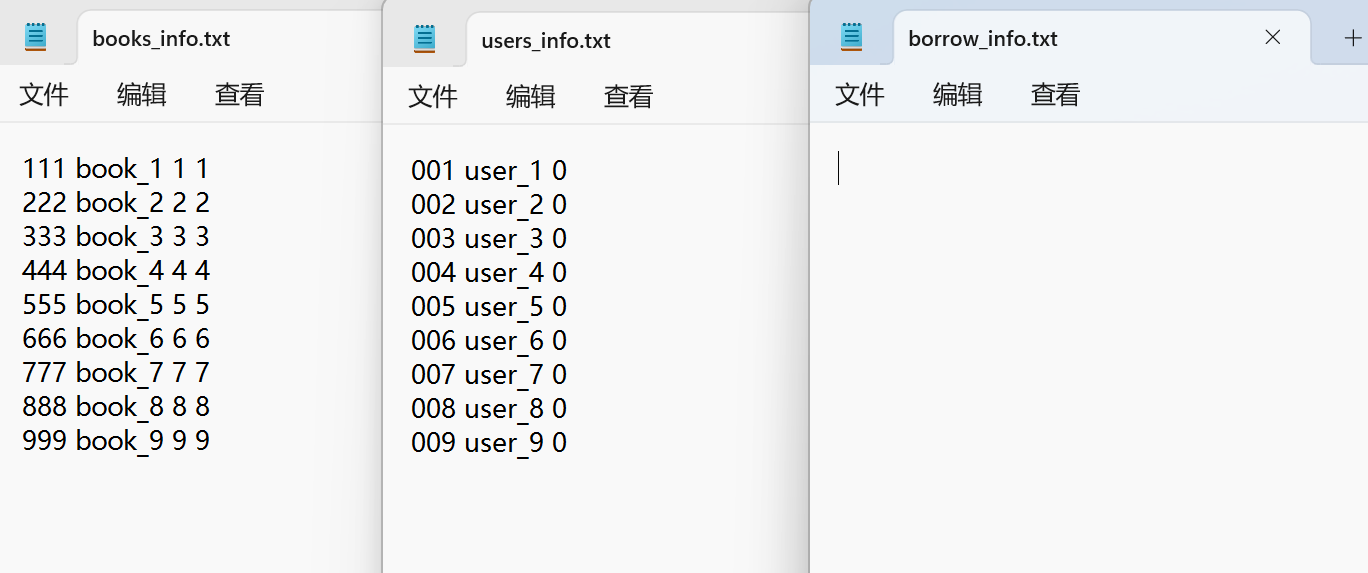
\includegraphics[width=0.95\textwidth]{src/before.png}
        \caption{运行程序前数据库中的信息}    
    \end{figure}
    
    \begin{figure}[!htbp]
        \centering
        \begin{subfigure}{0.34\textwidth}
            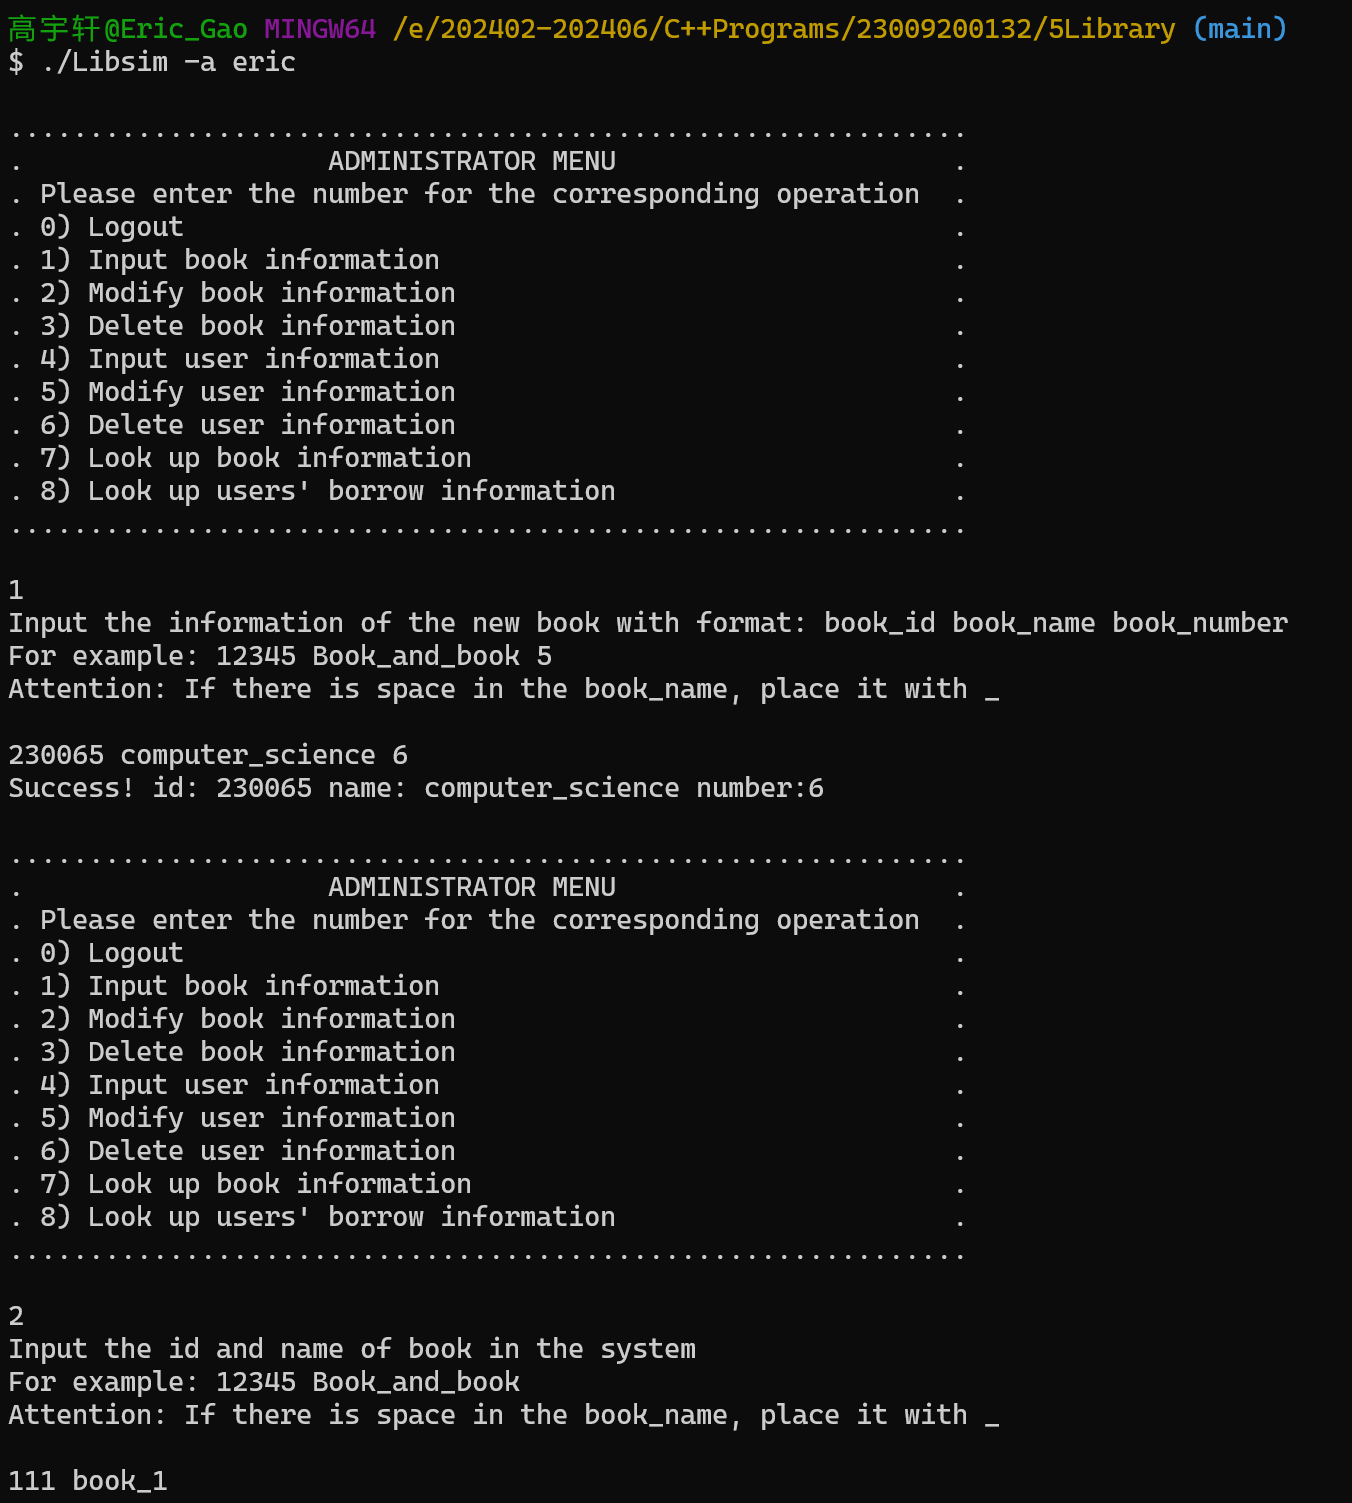
\includegraphics[width=\linewidth]{src/admin01.png}
            \caption{以管理员身份运行程序的界面}
        \end{subfigure}
        \begin{subfigure}{0.64\textwidth}
            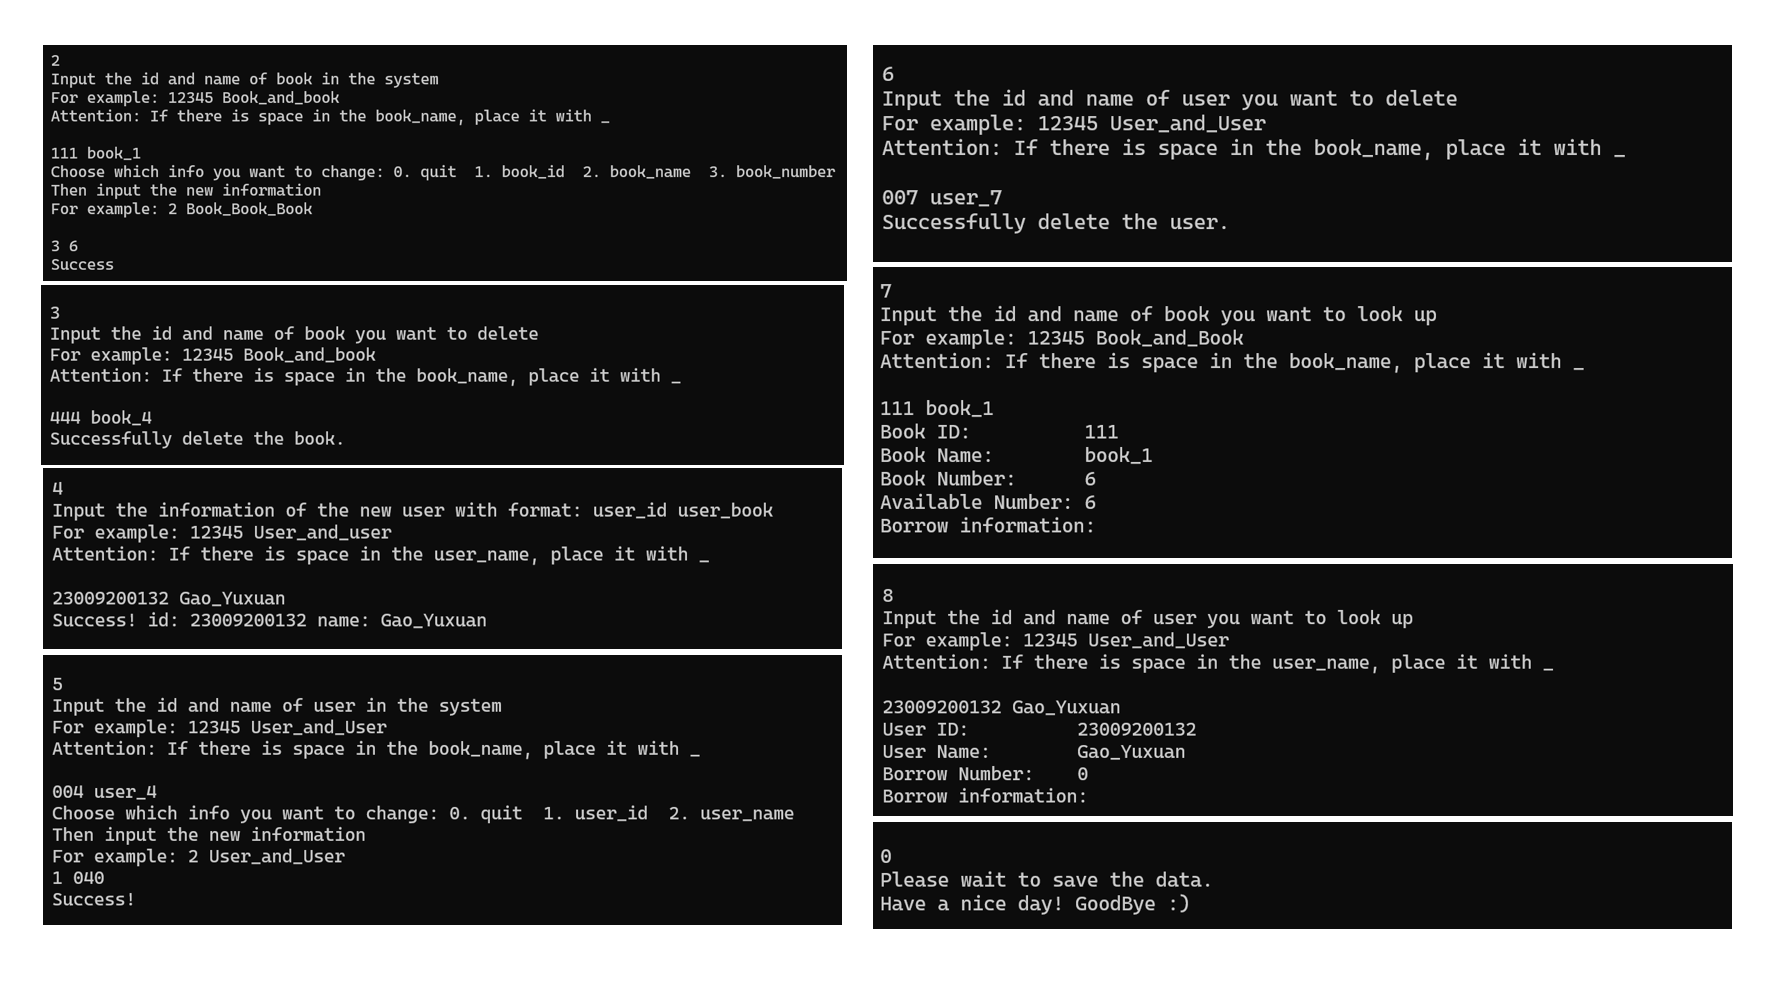
\includegraphics[width=\linewidth]{src/admin00.png}
            \caption{以管理员身份进行操作}
        \end{subfigure}
        \caption{以管理员身份运行程序}
    \end{figure}
    
    \begin{figure}[!htbp] % 'h' 表示将图片放置在当前位置
        \centering
        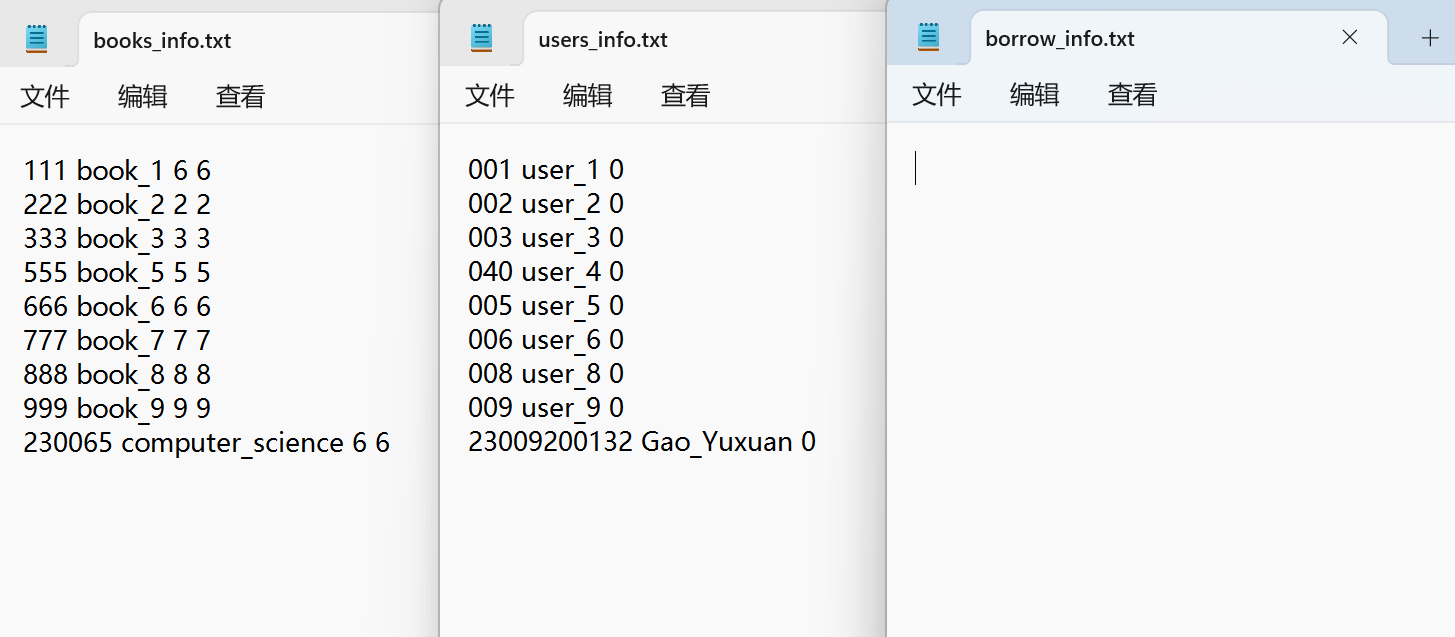
\includegraphics[width=0.9\textwidth]{src/admin_result.png}
        \caption{以管理员身份操作之后的数据库信息}    
    \end{figure}
    
    \begin{figure}[!htbp]
        \centering
        \begin{subfigure}{0.34\textwidth}
            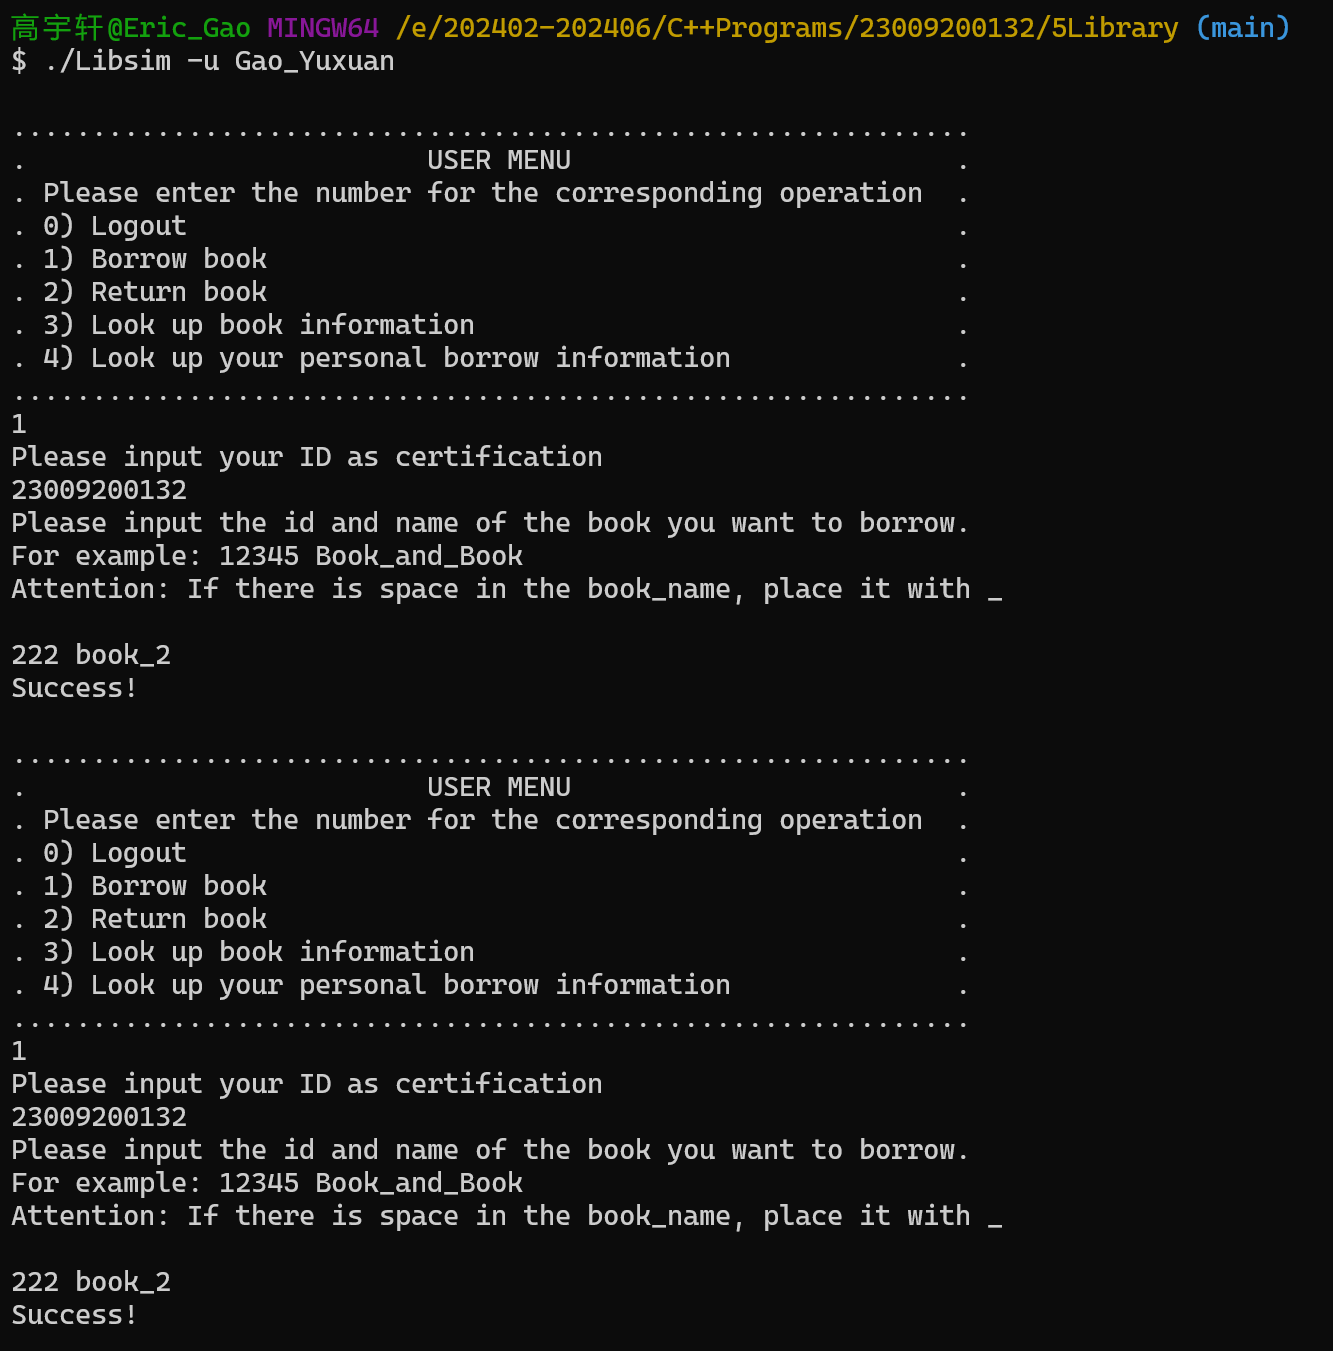
\includegraphics[width=\linewidth]{src/user01.png}
            \caption{以用户身份运行程序的界面}
        \end{subfigure}
        \begin{subfigure}{0.64\textwidth}
            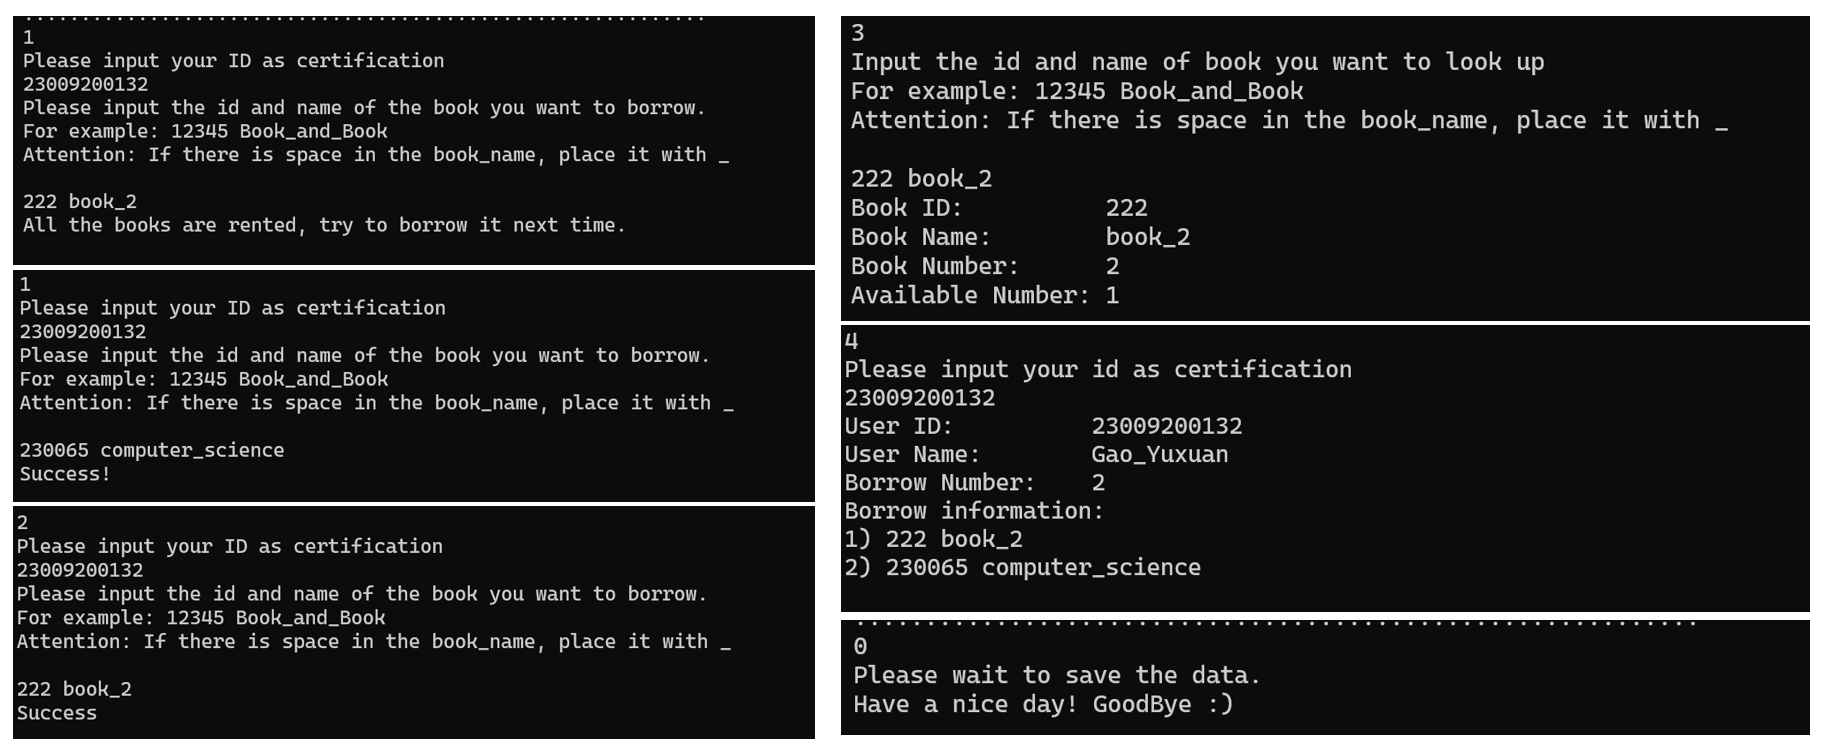
\includegraphics[width=\linewidth]{src/user00.png}
            \caption{以用户身份进行操作}
        \end{subfigure}
        \caption{以用户身份运行程序}
    \end{figure}
    
    \begin{figure}[!htbp] % 'h' 表示将图片放置在当前位置
        \centering
        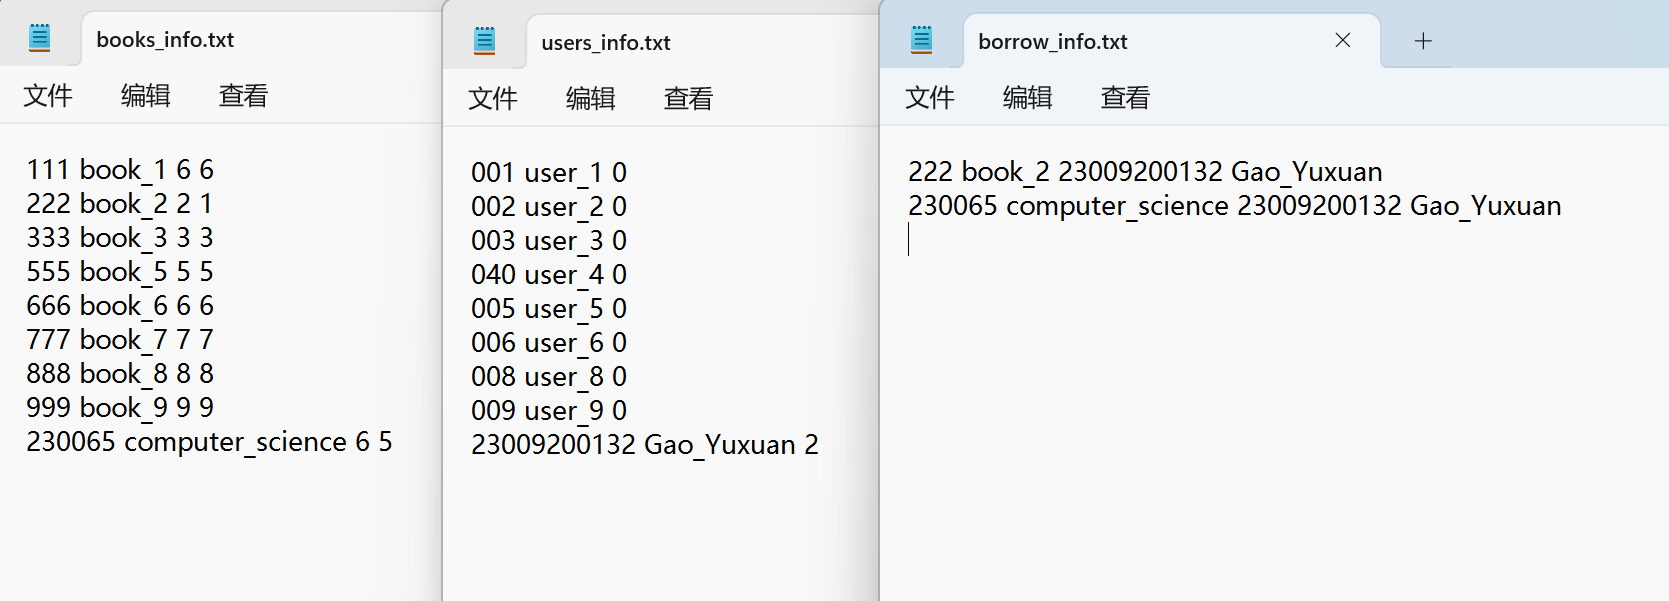
\includegraphics[width=0.9\textwidth]{src/user_result.png}
        \caption{以用户身份操作之后的数据库信息}    
    \end{figure}
    
    \section{总结}
    
    \subsection{程序结果分析}
    通过以上的集成测试,我们可以看出,不论是管理员录入、修改、删除书本或用户信息,还是用户借书、还书,都能够顺利地同步数据。
    
    \subsection{程序的不足与改进方案}
    \begin{enumerate}
        \item[1)] 每一次重新开始运行程序时都要先将全部的数据信息载入内存,然后再进行处理,这对内存造成了很大的负担,在以后的改进中应当想办法优化这一点,直接在数据库中进行增删改查。
        \item[2)] 使用链表存储数据时,线性的查询速度在数据量较大时会非常慢,可以使用B+树等数据结构存储数据,从而大幅度加快数据处理的速度。
    \end{enumerate}
    

    
    
\end{document}
